%
% CSE Electronic Homework Template
% Last modified 8/23/2018 by Jeremy Buhler

\documentclass[11pt]{article}
\usepackage[left=0.7in,right=0.7in,top=1in,bottom=0.7in]{geometry}
\usepackage{fancyhdr} % for header
\usepackage{graphicx} % for figures
\usepackage{amsmath}  % for extended math markup
\usepackage{amssymb}
\usepackage[bookmarks=false]{hyperref} % for URL embedding
\usepackage[noend]{algpseudocode} % for pseudocode
\usepackage[plain]{algorithm} % float environment for algorithms

%%%%%%%%%%%%%%%%%%%%%%%%%%%%%%%%%%%%%%%%%%%%%%%%%%%%%%%%%%%%%%%%%%%%%%
% STUDENT: modify the following fields to reflect your
% name/ID, the current homework, and the current problem number

% Example: 
%\newcommand{\StudentName}{Jeremy Buhler}
%\newcommand{\StudentID{123456}

\newcommand{\StudentName}{Dingyu Wang (Howard)}
\newcommand{\StudentID}{COMP 642: Machine Learning}
\newcommand{\HomeworkNumber}{5}

%%%%%%%%%%%%%%%%%%%%%%%%%%%%%%%%%%%%%%%%%%%%%%%%%%%%%%%%%%%%%%%%%%%%%%%%
% You can pretty much leave the stuff up to the next line of %%'s alone.

% create header and footer for every page
\pagestyle{fancy}
\fancyhf{}
\lhead{\textbf{\StudentName}}
\chead{\textbf{\StudentID}}
\rhead{\textbf{HW \HomeworkNumber}}
\cfoot{\thepage}

% preferred pseudocode style
\algrenewcommand{\algorithmicprocedure}{}
\algrenewcommand{\algorithmicthen}{}

% ``do { ... } while (cond)''
\algdef{SE}[DOWHILE]{Do}{doWhile}{\algorithmicdo}[1]{\algorithmicwhile\ #1}%

% ``for (x in y ... z)''
\newcommand{\ForRange}[3]{\For{#1 \textbf{in} #2 \ \ldots \ #3}}

% these are common math formatting commands that aren't defined by default
\newcommand{\union}{\cup}
\newcommand{\isect}{\cap}
\newcommand{\ceil}[1]{\ensuremath \left\lceil #1 \right\rceil}
\newcommand{\floor}[1]{\ensuremath \left\lfloor #1 \right\rfloor}

%%%%%%%%%%%%%%%%%%%%%%%%%%%%%%%%%%%%%%%%%%%%%%%%%%%%%%%%%%%%%%%%%%%%%%
\usepackage[utf8]{inputenc}
\usepackage[english]{babel}
\setlength{\parindent}{0em}
\setlength{\parskip}{1em}
 \usepackage{pythonhighlight}
\usepackage{graphicx}
\graphicspath{ {./images/} }


\begin{document}

1) \\
mean: 
$
\begin{vmatrix}
2 \\
3
\end{vmatrix}
\qquad
$
covariant:
$ 
\begin{vmatrix}
2 & 2 \\
2 & 3
\end{vmatrix}
$ \\ 

characteristic polynomial:
$ 
\begin{vmatrix}
2 - \lambda & 2 \\
2 & 3 - \lambda
\end{vmatrix}
= 
(2-\lambda)(3-\lambda) - (2)(2) = \lambda^2 - 5\lambda + 2
$ \\

$
\lambda_1, \lambda_2 =\frac{5\pm\sqrt{(-5)^2-4(1)(2)}}{2(1)}
$ \\

$
\lambda_1 = \frac{5-\sqrt{17}}{2} = 0.438 \qquad \lambda_2 = \frac{5+\sqrt{17}}{2} = 4.56
$ \\

$
A - \lambda_1 I = 
\begin{vmatrix}
 \frac{\sqrt{17} - 1}{2} & 2 \\
2 &  \frac{\sqrt{17} + 1}{2} 
\end{vmatrix}
 \qquad 
 A- \lambda_2 I =  
 \begin{vmatrix}
 \frac{-\sqrt{17} - 1}{2} & 2 \\
2 &  \frac{-\sqrt{17} + 1}{2} 
\end{vmatrix}
$ \\ 

$
v_1 = 
\begin{vmatrix}
\frac{-\sqrt{17}-1}{4} \\ 
1
\end{vmatrix} 
= 
\begin{vmatrix}
-1.281 \\ 
1
\end{vmatrix} 
\qquad
v_2 = 
\begin{vmatrix}
\frac{\sqrt{17}-1}{4} \\ 
1
\end{vmatrix}
= 
\begin{vmatrix}
0.781 \\ 
1
\end{vmatrix} 
$ \\


2) \\
The variance explained by the first component 4.5616/(4.5616+0.4384) = 0.9123.

3) \\
The variance explained by the second component is 0.4384/(4.5616+0.4384)=0.0877.

4) \\

Code is included in the Jupyter notebook. \\

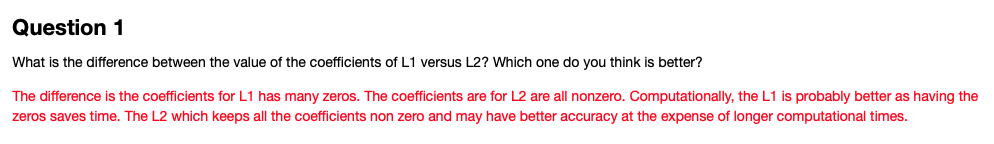
\includegraphics[scale=0.33]{Q1} \\
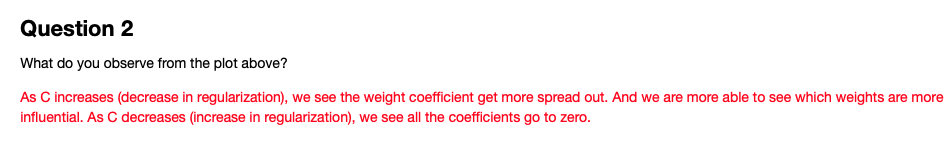
\includegraphics[scale=0.33]{Q2} \\
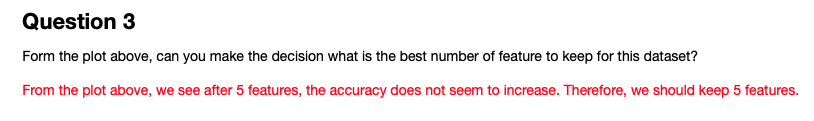
\includegraphics[scale=0.33]{Q3} \\
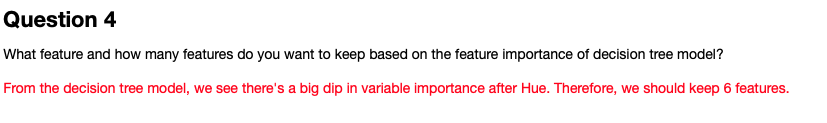
\includegraphics[scale=0.33]{Q4} \\

\includegraphics[scale=0.33]{Q5} \\

\end{document}

